\section{Visione d'insieme}
In questa sezione sono presenti i risultati ottenuti durante lo sviluppo del progetto, confrontandoli con gli obiettivi iniziali e valutando il successo del progetto stesso.
\subsection{Prodotto finale}
Il prodotto finale del progetto è un sistema \textit{honeypot} modulare e scalabile, in grado di monitorare e analizzare tentativi di attacco su vari servizi di rete.
Nelle figure seguenti sono mostrate le principali componenti del sistema, che spaziano dalla configurazione iniziale del \textit{logger}, alla gestione del database tramite \textit{InfluxDB}, fino alla visualizzazione dei dati attraverso le dashboard interattive fornite da \textit{Grafana}.
\begin{figure}[H]
    \begin{center}
    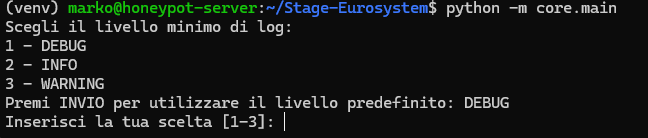
\includegraphics[width=\textwidth]{img/environment.png}
    \caption{Scelta del livello minimo del \textit{logger} al momento dell'inizializzazione.}
    \label{fig:environment}
    \end{center}
\end{figure}
\begin{figure}[H]
    \begin{center}
    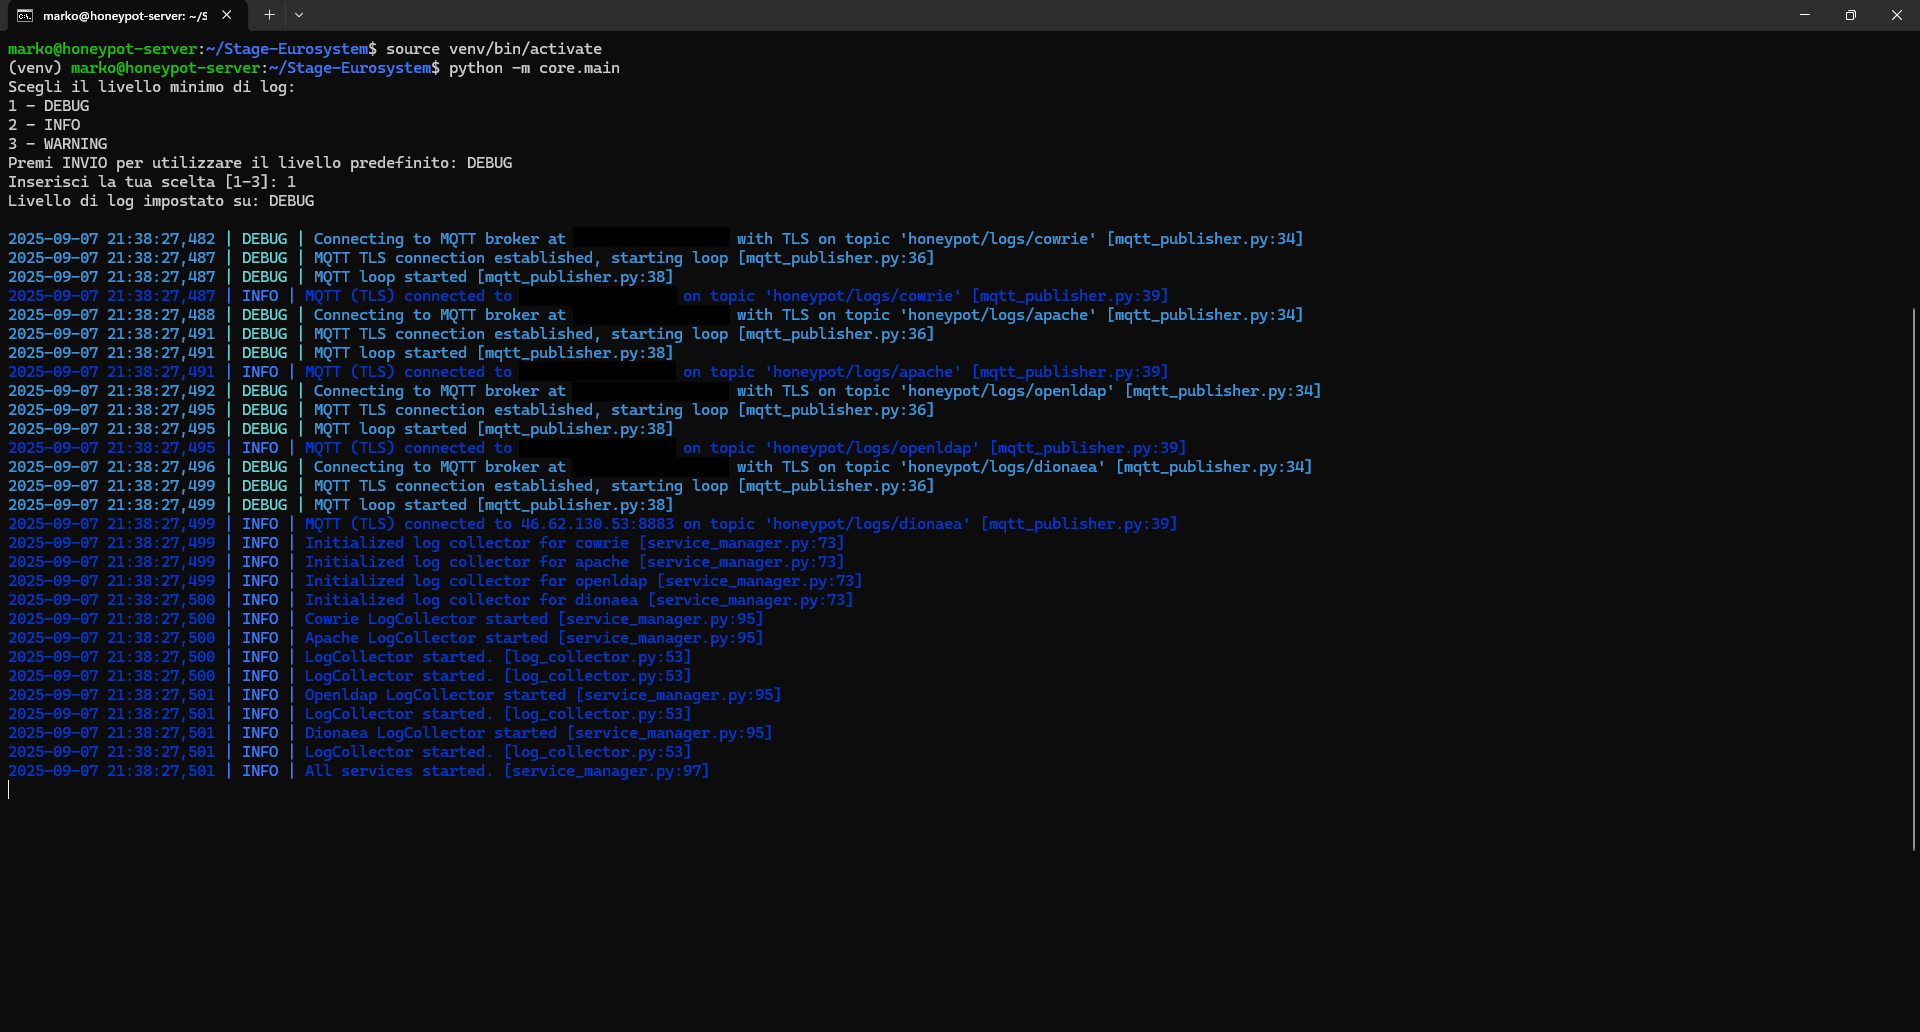
\includegraphics[width=\textwidth]{img/logger.png}
    \caption{Esempio di \textit{logger} in funzione in modalità \textit{debug}.}
    \label{fig:logger}
    \end{center}
\end{figure}
\begin{figure}[H]
    \begin{center}
    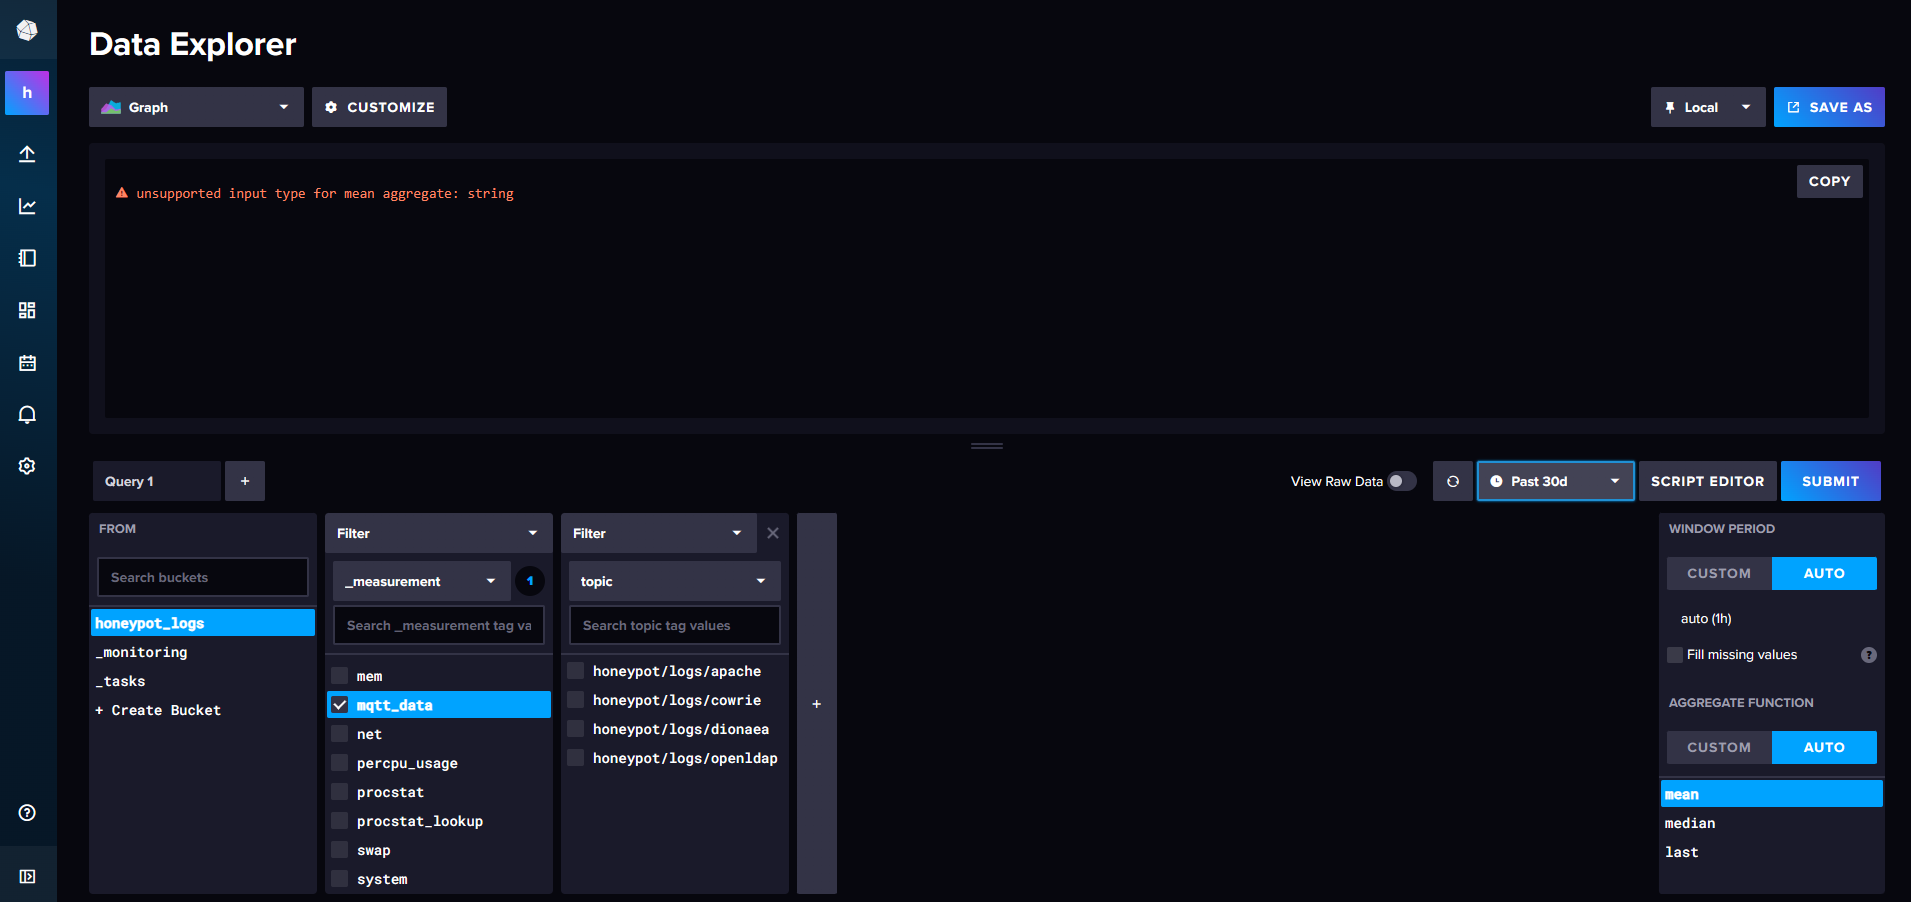
\includegraphics[width=\textwidth]{img/influxdb.png}
    \caption{Interfaccia web di \textit{InfluxDB} per la gestione del \textit{database}.}
    \label{fig:influxdb}
    \end{center}
\end{figure}
\begin{figure}[H]
    \begin{center}
    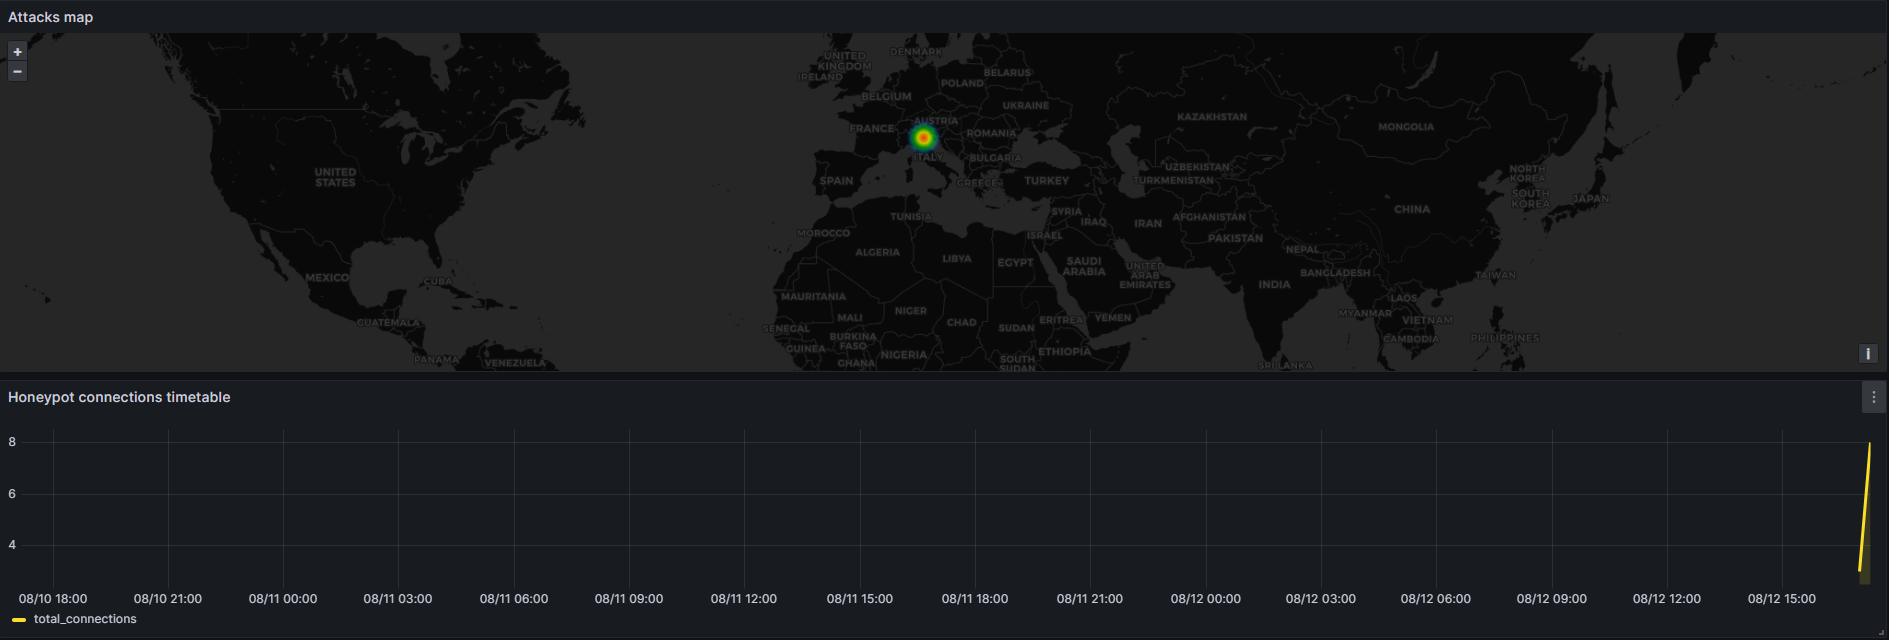
\includegraphics[width=\textwidth]{img/grafana-1.png}
    \caption{Esempio di \textit{dashboard} di \textit{Grafana} per la visualizzazione dei dati raccolti dall'\textit{honeypot}.}
    \label{fig:grafana-1}
    \end{center}
\end{figure}
\begin{figure}[H]
    \begin{center}
    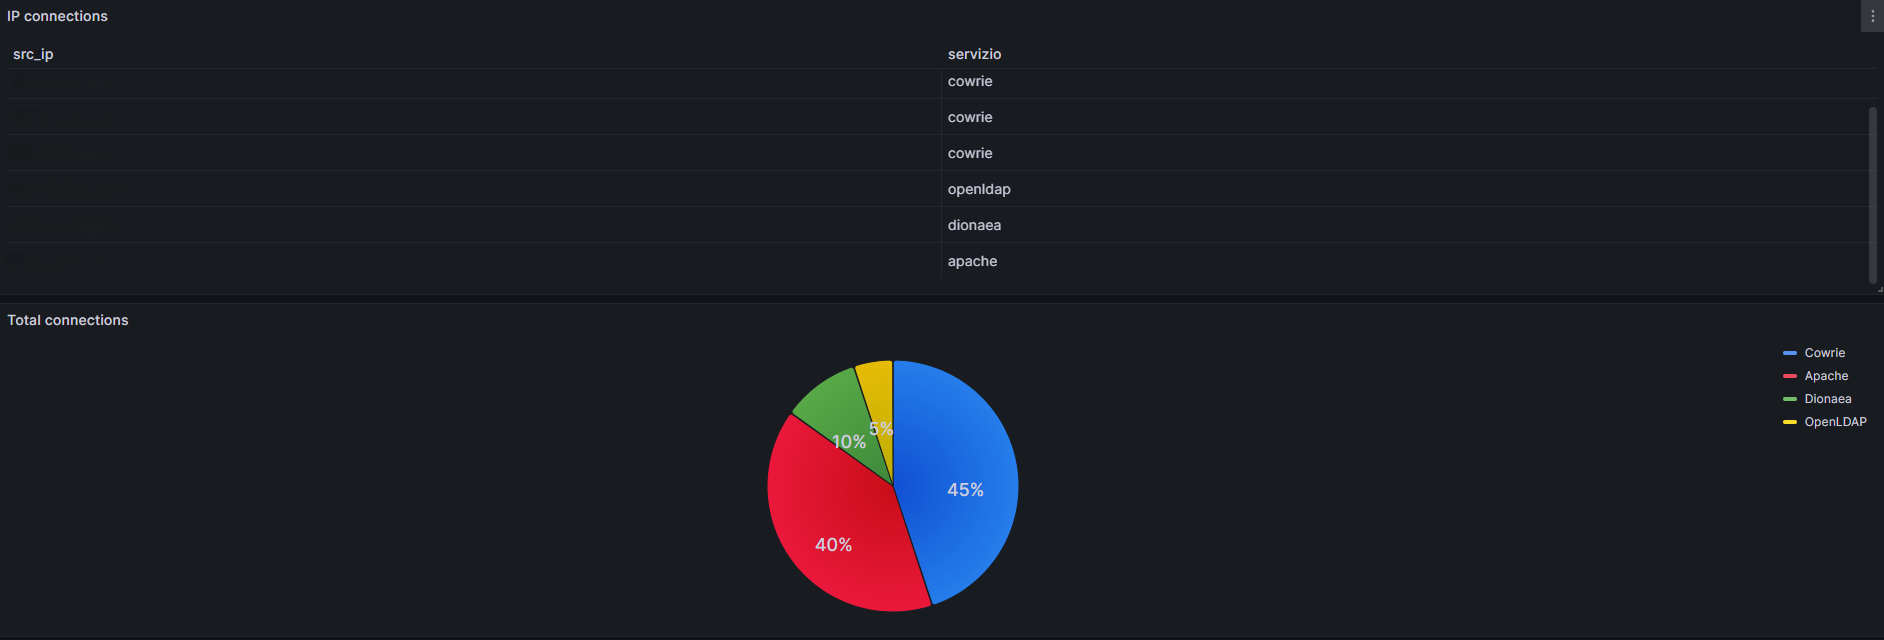
\includegraphics[width=\textwidth]{img/grafana-2.png}
    \caption{Esempio di \textit{dashboard} di \textit{Grafana} per la visualizzazione dei dati raccolti dall'\textit{honeypot}.}
    \label{fig:grafana-2}
    \end{center}
\end{figure}
\begin{figure}[H]
    \begin{center}
    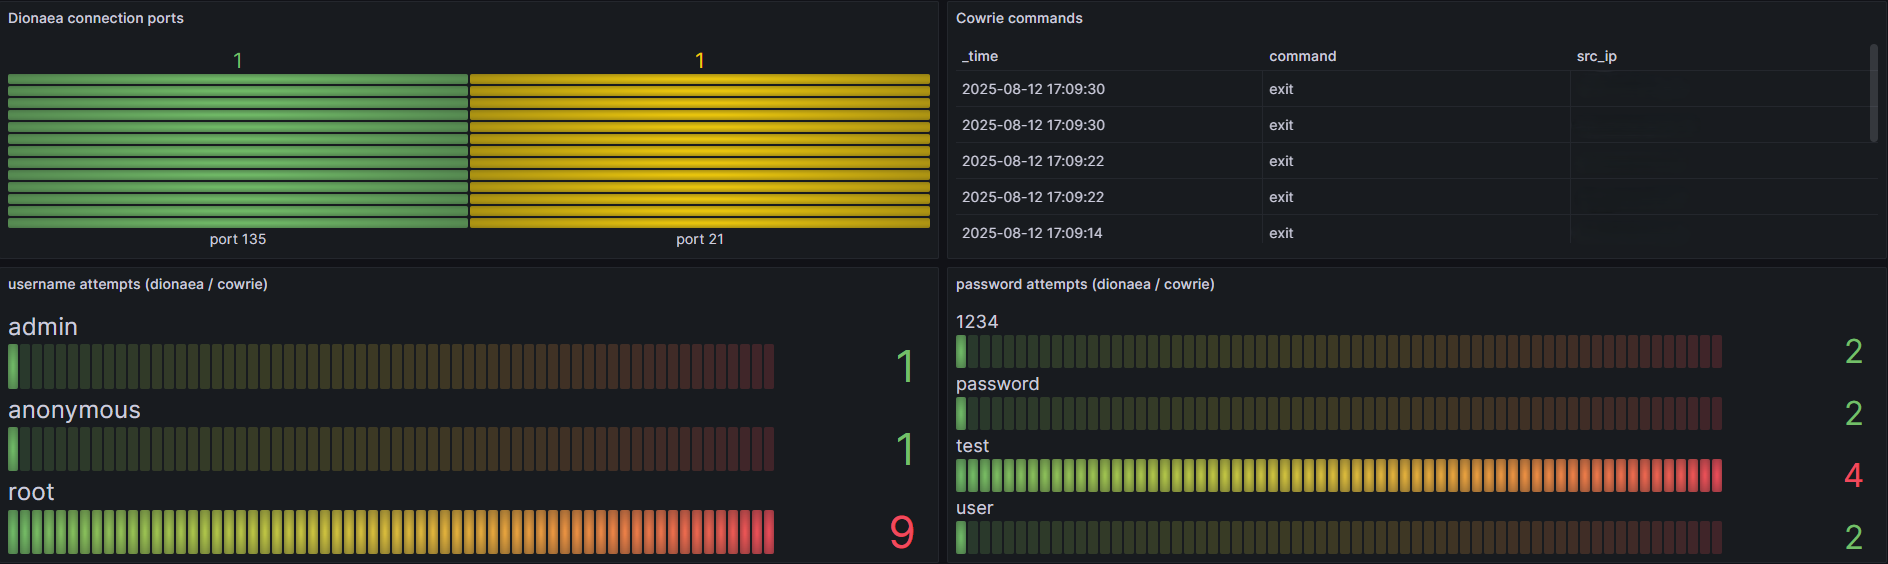
\includegraphics[width=\textwidth]{img/grafana-3.png}
    \caption{Esempio di \textit{dashboard} di \textit{Grafana} per la visualizzazione dei dati raccolti dall'\textit{honeypot}.}
    \label{fig:grafana-3}
    \end{center}
\end{figure}
Gli indirizzi \textit{IP} sono opportunamente mascherati per motivi di sicurezza.